\setcounter{ExampleCounter}{1}
In this section, we'll briefly state a few \textbf{identities}, including De Morgan's laws that we observed in the last section.\\

We won't see any rigorous proofs of these identities, but if you're curious, the way to prove that two sets $A$ and $B$ are equal is to show that every element in each of them is also in the other; in other words, to show that
\[A \subseteq B \ \ \textrm{ and } \ \ B \subseteq A.\]

To do so, we would take an element from one set and show that it must belong to the other set, and then pick an element from the second set and show that it must belong to the first.\\

Instead of doing proofs like that, we'll simply illustrate each identity with an example and with an appropriate Venn diagram.

\subsection{Associative Identities}
The associative identities essentially state that the placement of parentheses doesn't matter when we're only doing one kind of operation (union or intersection):
\begin{align*}
(A \cup B) \cup C &= A \cup (B \cup C)\\
(A \cap B) \cap C &= A \cap (B \cap C)
\end{align*}

Think about the first one, for instance, and let's see if we can make sense of it.  It says that if we start with $A$, add in the elements of $B$, and then add in the elements of $C$, we'd get the same result as if we start with $B$, add in the elements of $C$, and finally add in the elements of $A$.  Either way, we get the elements that are in any of the three sets.

\begin{center}
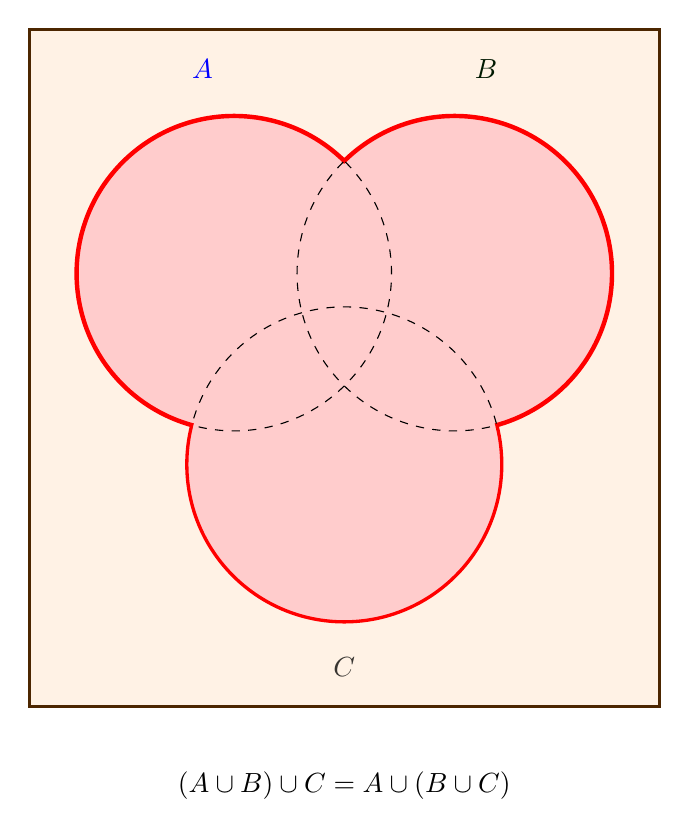
\begin{tikzpicture}
  \draw [very thick,color=orange!30!black, fill=orange, fill opacity=0.1] (-4cm,-5.5cm) rectangle (4cm,3.1cm);

  \draw [very thick,color=red, fill=red!20] (0,-2.425) circle (2cm);
  \draw [very thick,color=red!20, fill=red!20] (-1.4,0) circle (2cm);
  \draw [very thick,color=red!20, fill=red!20] (1.4,0) circle (2cm);
  
  \draw [yshift=2.6cm,xshift=-1.8cm] node {\color{blue} $A$};
  \draw [yshift=2.6cm,xshift=1.8cm] node {\color{green!10!black} $B$};
  \draw [yshift=-5cm,xshift=0cm] node {\color{yellow!10!black} $C$};
  
  \draw [yshift=-6.5cm,xshift=0cm] node {$(A \cup B) \cup C = A \cup (B \cup C)$};
  
  \draw [ultra thick, color=red] (-1.4,0) ++(45:2) arc (45:255:2);
  \draw [ultra thick, color=red] (1.4,0) ++(135:2) arc (135:-75:2);
  
  \draw [dashed,color=black] (-1.4,0) ++(45:2) arc (45:-105:2);
  \draw [dashed,color=black] (1.4,0) ++(135:2) arc (135:285:2);
  \draw [dashed,color=black] (0,-2.425) ++(15:2) arc (15:165:2);
  
\end{tikzpicture}
\end{center}

\vfill
\pagebreak

The second is similar: whether you start by intersecting $A$ and $B$, and then intersect that with $C$, or start by intersecting $B$ and $C$, what you ultimately find is all the elements that belong to all three sets at once.  For instance, if you start by intersecting $A$ and $B$, you start with $A$, remove any elements that don't belong to $B$, and finally remove any elements that don't belong to $C$.

\begin{center}
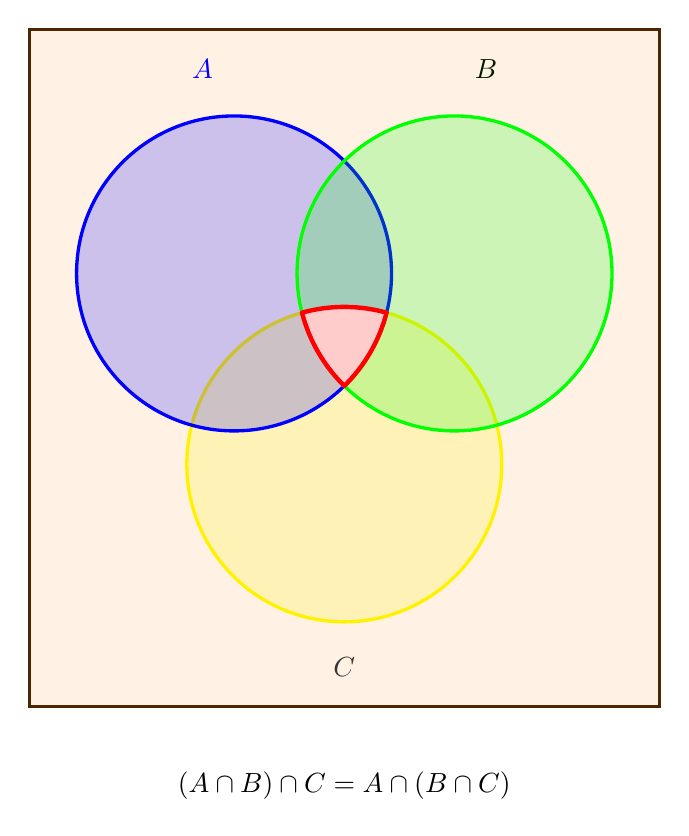
\begin{tikzpicture}
  \draw [very thick,color=orange!30!black, fill=orange, fill opacity=0.1] (-4cm,-5.5cm) rectangle (4cm,3.1cm);

  \draw [very thick,color=yellow, fill=yellow, fill opacity=0.2] (0,-2.425) circle (2cm);
  \draw [very thick,color=blue, fill=blue, fill opacity=0.2] (-1.4,0) circle (2cm);
  \draw [very thick,color=green, fill=green, fill opacity=0.2] (1.4,0) circle (2cm);
  
  \draw [yshift=2.6cm,xshift=-1.8cm] node {\color{blue} $A$};
  \draw [yshift=2.6cm,xshift=1.8cm] node {\color{green!10!black} $B$};
  \draw [yshift=-5cm,xshift=0cm] node {\color{yellow!10!black} $C$};
  
  \draw [yshift=-6.5cm,xshift=0cm] node {$(A \cap B) \cap C = A \cap (B \cap C)$};
  
  \node (a) at (0.5,-0.5) {};
  \node (b) at (-0.5,-0.5) {};
  \node (c) at (0,-1.37) {};
  \draw [ultra thick,fill=red!20,red!20] (a.center) -- (b.center) -- (c.center) -- (a.center) -- cycle;
  
  \draw [ultra thick,color=red,fill=red!20] (-1.4,0) ++(314:2) node(c){} arc (314:346:2);
  \draw [ultra thick,color=red,fill=red!20] (1.4,0) ++(194:2) node(b){} arc (194:226:2);
  \draw [ultra thick,color=red,fill=red!20] (0,-2.425) ++(74:2) node(a){} arc (74:106:2);
  
  
\end{tikzpicture}
\end{center}

\begin{example}[https://www.youtube.com/watch?v=-sCqd8YgN-s]{Associative Identities}
Suppose we have the following sets:
\begin{align*}
A &= \{1,2,3,4,5\}\\
B &= \{2,4,6,8,9\}\\
C &= \{1,3,9,10,11\}
\end{align*}
Illustrate the associative identities with these sets.\\

\begin{enumerate}[(a)]
\item First, show that $(A \cup B) \cup C = A \cup (B \cup C)$ in this example:
\begin{align*}
A \cup B &= \{1,2,3,4,5,6,8,9\}\\
(A \cup B) \cup C &= \{1,2,3,4,5,6,8,9,10,11\}\\
&\\
B \cup C &= \{1,2,3,4,6,8,9,10,11\}\\
A \cup (B \cup C) &= \{1,2,3,4,5,6,8,9,10,11\}
\end{align*}

\item Then, show that $(A \cap B) \cap C = A \cap (B \cap C)$:
\begin{align*}
A \cap B &= \{2,4\}\\
(A \cap B) \cap C &= \varnothing\\
&\\
B \cap C &= \{9\}\\
A \cap (B \cap C) &= \varnothing
\end{align*}
\end{enumerate}

In both cases, the associative identity held true.
\end{example}


\subsection{Distributive Identities}
If you remember from your algebra classes, you can distribute something like \[2(x+4) = 2x+8\] by applying the multiplication to both terms inside the parentheses.  We can do something similar with set operations, where we can distribute one operation across parentheses where the other is used:
\begin{align*}
A \cap (B \cup C) &= (A \cap B) \cup (A \cap C)\\
A \cup (B \cap C) &= (A \cup B) \cap (A \cup C)
\end{align*}

The best way to make sense of these is probably to use the Venn diagrams below:

\begin{center}
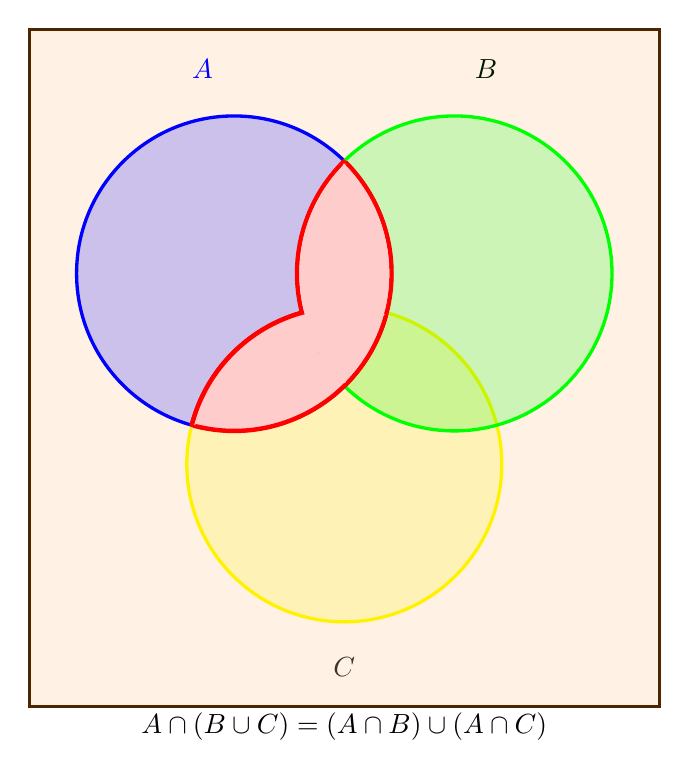
\begin{tikzpicture}
  \draw [very thick,color=orange!30!black, fill=orange, fill opacity=0.1] (-4cm,-5.5cm) rectangle (4cm,3.1cm);

  \draw [very thick,color=yellow, fill=yellow, fill opacity=0.2] (0,-2.425) circle (2cm);
  \draw [very thick,color=blue, fill=blue, fill opacity=0.2] (-1.4,0) circle (2cm);
  \draw [very thick,color=green, fill=green, fill opacity=0.2] (1.4,0) circle (2cm);
  
  \draw [yshift=2.6cm,xshift=-1.8cm] node {\color{blue} $A$};
  \draw [yshift=2.6cm,xshift=1.8cm] node {\color{green!10!black} $B$};
  \draw [yshift=-5cm,xshift=0cm] node {\color{yellow!10!black} $C$};
  
  \draw [yshift=-5.75cm,xshift=0cm] node {$A \cap (B \cup C) = (A \cap B) \cup (A \cap C)$};
  
  %\node (a) at (0.5,-0.5) {};
  %\node (b) at (-0.5,-0.5) {};
  %\node (c) at (0,-1.37) {};
  %\draw [ultra thick,fill=red!20,red!20] (a.center) -- (b.center) -- (c.center) -- (a.center) -- cycle;
  
  %\draw [ultra thick,color=red,fill=red!20] (-1.4,0) ++(314:2) node(c){} arc (314:346:2);
  %\draw [ultra thick,color=red,fill=red!20] (1.4,0) ++(194:2) node(b){} arc (194:226:2);
  %\draw [ultra thick,color=red,fill=red!20] (0,-2.425) ++(74:2) node(a){} arc (74:106:2);
  
  \draw [ultra thick,color=red!20] (0,-1.414) -- (0,1.414);
  \draw [ultra thick,color=red,fill=red!20] (-1.4,0) ++(45:2) arc (45:-45:2);
  \draw [ultra thick,color=red,fill=red!20] (1.4,0) ++(134:2) arc (134:226:2);
  
  
  \draw [ultra thick,color=red,fill=red!20] (0,-2.425) ++(75:2) node(b){} arc (75:165:2) node(a){};
  \draw [ultra thick,color=red,fill=red!20] (-1.4,0) ++(-15:2) arc (-15:-105:2);
  \draw [ultra thick,color=red!20] (b) -- (a.center);
  \draw [ultra thick,color=red,fill=red!20] (0,-2.425) ++(74:2) arc (74:166:2);
  
  \draw [thick,color=red!20] (0,-1.2) -- (0,0);
  \draw [color=red!20,fill=red!20] (-1.4,0) ++(45:1.965) arc (45:-45:1.965);
  \draw [color=red!20,fill=red!20] (1.4,0) ++(135:1.965) arc (135:225:1.965);
  
\end{tikzpicture}
\end{center}

\vspace{0.3in}

\begin{center}
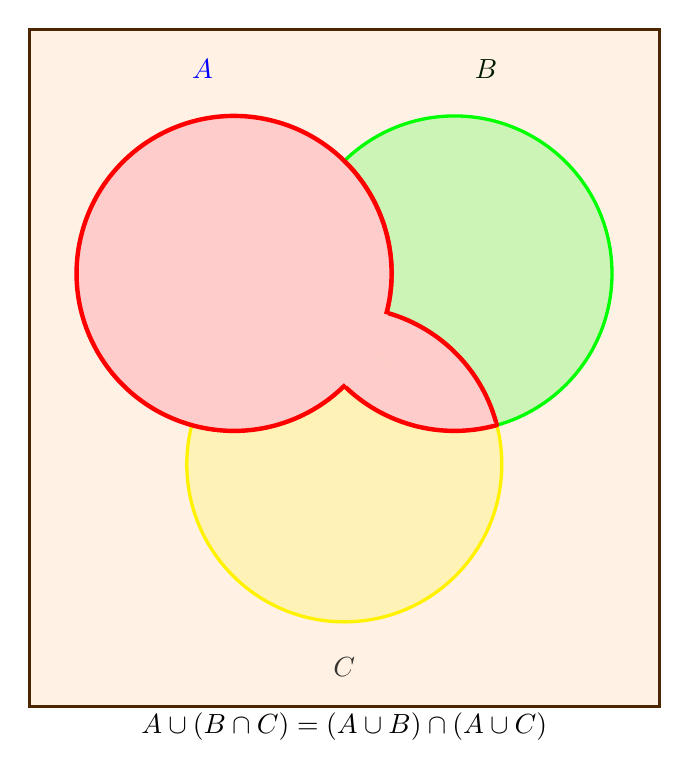
\begin{tikzpicture}
  \draw [very thick,color=orange!30!black, fill=orange, fill opacity=0.1] (-4cm,-5.5cm) rectangle (4cm,3.1cm);

  \draw [very thick,color=yellow, fill=yellow, fill opacity=0.2] (0,-2.425) circle (2cm);
  %\draw [very thick,color=blue, fill=blue, fill opacity=0.2] (-1.4,0) circle (2cm);
  \draw [very thick,color=green, fill=green, fill opacity=0.2] (1.4,0) circle (2cm);
  
  \draw [yshift=2.6cm,xshift=-1.8cm] node {\color{blue} $A$};
  \draw [yshift=2.6cm,xshift=1.8cm] node {\color{green!10!black} $B$};
  \draw [yshift=-5cm,xshift=0cm] node {\color{yellow!10!black} $C$};
  
  \draw [yshift=-5.75cm,xshift=0cm] node {$A \cup (B \cap C) = (A \cup B) \cap (A \cup C)$};
  
  %\node (a) at (0.5,-0.5) {};
  %\node (b) at (-0.5,-0.5) {};
  %\node (c) at (0,-1.37) {};
  %\draw [ultra thick,fill=red!20,red!20] (a.center) -- (b.center) -- (c.center) -- (a.center) -- cycle;
  
  %\draw [ultra thick,color=red,fill=red!20] (-1.4,0) ++(314:2) node(c){} arc (314:346:2);
  %\draw [ultra thick,color=red,fill=red!20] (1.4,0) ++(194:2) node(b){} arc (194:226:2);
  %\draw [ultra thick,color=red,fill=red!20] (0,-2.425) ++(74:2) node(a){} arc (74:106:2);
  
  \draw [ultra thick,color=red!20] (0,-1.414) -- (0,1.414);
  \draw [ultra thick,color=red,fill=red!20] (-1.4,0) ++(45:2) arc (45:-45:2);
  \draw [ultra thick,color=red,fill=red!20] (1.4,0) ++(134:2) arc (134:226:2);
  
  
  \draw [ultra thick,color=red,fill=red!20] (0,-2.425) ++(14:2) node(b){} arc (14:105:2) node(a){};
  \draw [ultra thick,color=red,fill=red!20] (1.4,0) ++(195:2) arc (195:286:2);
  \draw [ultra thick,color=red!20] (b.north west) -- (a.center);
  %\draw [ultra thick,color=red,fill=red!20] (0,-2.425) ++(74:2) arc (74:166:2);
  
  %\draw [thick,color=red!20] (0,-1.2) -- (0,0);
  %\draw [color=red!20,fill=red!20] (-1.4,0) ++(45:1.965) arc (45:-45:1.965);
  %\draw [color=red!20,fill=red!20] (1.4,0) ++(135:1.965) arc (135:225:1.965);
  
  \draw [very thick,color=red!20, fill=red!20] (-1.4,0) circle (2cm);
  \draw [ultra thick,color=red] (-1.4,0) ++(-15:2) arc (-15:315:2);
  
\end{tikzpicture}
\end{center}
\vfill
\pagebreak

\begin{example}[https://www.youtube.com/watch?v=d6WMaLCszKM]{Distributive Identities}
Suppose we have the following sets:
\begin{align*}
A &= \{1,2,3,4,5\}\\
B &= \{2,4,6,8,9\}\\
C &= \{1,3,9,10,11\}
\end{align*}
Illustrate the distributive identities with these sets.\\

\begin{enumerate}[(a)]
\item First, show that $A \cap (B \cup C) = (A \cap B) \cup (A \cap C)$ in this example:
\begin{align*}
B \cup C &= \{1,2,3,4,6,8,9,10,11\}\\
A \cap (B \cup C) &= \{1,2,3,4\}\\
&\\
A \cap B &= \{2,4\}\\
A \cap C &= \{1,3\}\\
(A \cap B) \cup (A \cap C) &= \{1,2,3,4\}
\end{align*}

\item Then, show that $A \cup (B \cap C) = (A \cup B) \cap (A \cup C)$:
\begin{align*}
B \cap C &= \{9\}\\
A \cup (B \cap C) &= \{1,2,3,4,5,9\}\\
&\\
A \cup B &= \{1,2,3,4,5,6,8,9\}\\
A \cup C &= \{1,2,3,4,5,9,10,11\}\\
(A \cup B) \cap (A \cup C) &= \{1,2,3,4,5,9\}
\end{align*}
\end{enumerate}

In both cases, the distributive identity held true.
\end{example}

\subsection{De Morgan's Laws}
We've already noted these in passing.  These are especially important when it comes to logic (for instance, in computer programming), which is closely linked with set theory.
\begin{align*}
(A \cup B)^c &= A^c \cap B^c\\
(A \cap B)^c &= A^c \cup B^c
\end{align*}

The\marginnote{The connection to logic is this: if you tell someone ``don't get bread or milk,'' what you're really saying is ``don't get bread, and don't get milk.''} first one basically says that the set of points that don't lie in either $A$ or $B$ is the same as the set of points that don't lie in $A$ and don't lie in $B$.

\begin{center}
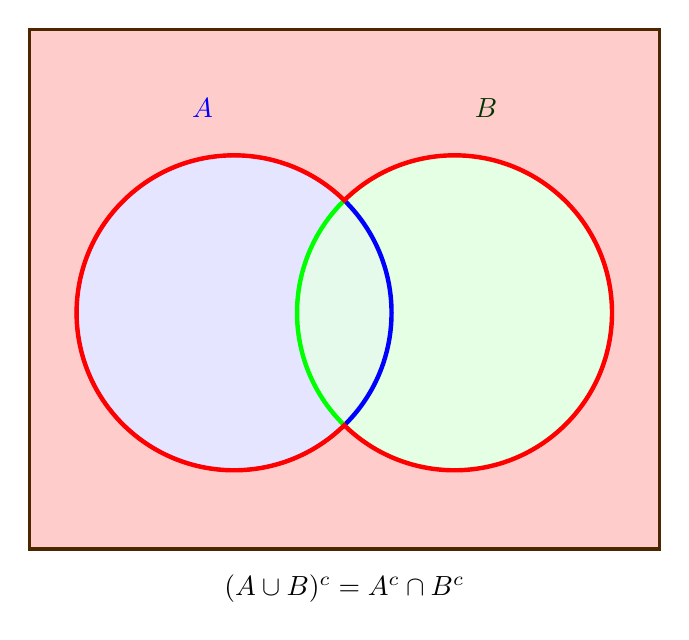
\begin{tikzpicture}
  \draw [very thick,color=orange!30!black, fill=red!20] (-4cm,-3cm) rectangle (4cm,3.6cm);

  \draw [very thick,color=blue, fill=blue!10] (-1.4,0) circle (2cm);
  \draw [very thick,color=green, fill=green!10] (1.4,0) circle (2cm);
  \draw [yshift=2.6cm,xshift=-1.8cm] node {\color{blue} $A$};
  \draw [yshift=2.6cm,xshift=1.8cm] node {\color{green!20!black} $B$};
  
  
  
  %\draw [ultra thick, color=red] (-1.4,0) ++(45:2) arc (45:315:2);
  %\draw [ultra thick, color=red] (1.4,0) ++(135:2) arc (135:-135:2);
  
  \draw [ultra thick,color=blue!20!green!10!white] (0,-1.414) -- (0,1.414);
  \draw [ultra thick,color=blue,fill=blue!20!green!10!white] (-1.4,0) ++(45:2) arc (45:-45:2);
  \draw [ultra thick,color=green,fill=blue!20!green!10!white] (1.4,0) ++(135:2) arc (135:225:2);
  \draw [ultra thick, color=red] (-1.4,0) ++(45:2) arc (45:315:2);
  \draw [ultra thick, color=red] (1.4,0) ++(135:2) arc (135:-135:2);
  %\draw [yshift=0cm,xshift=0cm] node {\color{red!20!black} $A \cap B$};
  
  \draw [yshift=-3.5cm,xshift=0cm] node {$(A \cup B)^c = A^c \cap B^c$};
  
\end{tikzpicture}
\end{center}

The second one says that points that don't lie in both $A$ and $B$ either don't lie in $A$ or don't lie in $B$.

\begin{center}
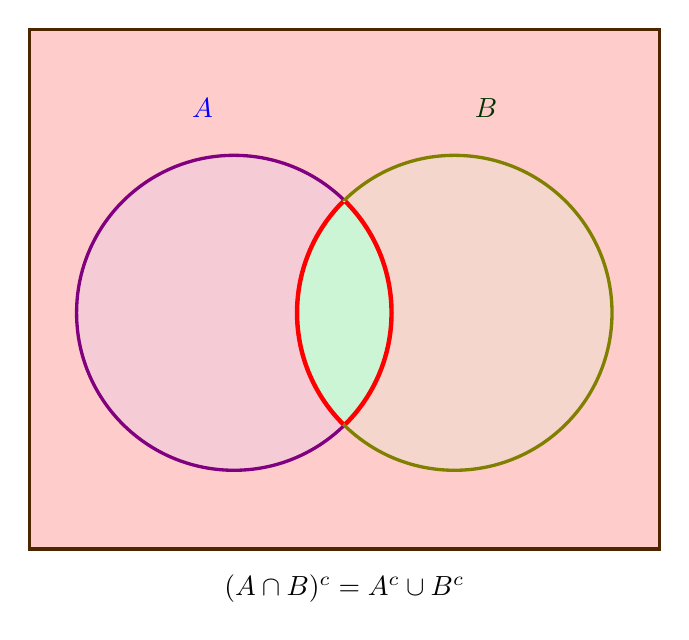
\begin{tikzpicture}
  \draw [very thick,color=orange!30!black, fill=red!20] (-4cm,-3cm) rectangle (4cm,3.6cm);

  \draw [very thick,color=blue!50!red, fill=blue!20!red!20] (-1.4,0) circle (2cm);
  \draw [very thick,color=green!50!red, fill=green!20!red!20] (1.4,0) circle (2cm);
  \draw [yshift=2.6cm,xshift=-1.8cm] node {\color{blue} $A$};
  \draw [yshift=2.6cm,xshift=1.8cm] node {\color{green!20!black} $B$};
  
  
  
  %\draw [ultra thick, color=red] (-1.4,0) ++(45:2) arc (45:315:2);
  %\draw [ultra thick, color=red] (1.4,0) ++(135:2) arc (135:-135:2);
  
  \draw [ultra thick,color=blue!20!green!20] (0,-1.414) -- (0,1.414);
  \draw [ultra thick,color=red,fill=blue!20!green!20] (-1.4,0) ++(45:2) arc (45:-45:2);
  \draw [ultra thick,color=red,fill=blue!20!green!20] (1.4,0) ++(135:2) arc (135:225:2);
  %\draw [yshift=0cm,xshift=0cm] node {\color{red!20!black} $A \cap B$};
  
  \draw [yshift=-3.5cm,xshift=0cm] node {$(A \cap B)^c = A^c \cup B^c$};
\end{tikzpicture}
\end{center}

\begin{example}[https://www.youtube.com/watch?v=fBOevsm5YrM]{De Morgan's Laws}
Suppose we have the following sets:
\begin{align*}
U &= \{a,b,c,d,e\}\\
A &= \{b,c\}\\
B &= \{a,c,e\}
\end{align*}
Illustrate De Morgan's laws with these sets.\\

\begin{enumerate}[(a)]
\item First, show that $(A \cup B)^c = A^c \cap B^c$ in this example:
\begin{align*}
A \cup B &= \{a,b,c,e\}\\
(A \cup B)^c &= \{d\}\\
&\\
A^c &= \{a,d,e\}\\
B^c &= \{b,d\}\\
A^c \cap B^c &= \{d\}
\end{align*}

\item Then, show that $(A \cap B)^c = A^c \cup B^c$:
\begin{align*}
A \cap B &= \{c\}\\
(A \cap B)^c &= \{a,b,d,e\}\\
&\\
A^c &= \{a,d,e\}\\
B^c &= \{b,d\}\\
A^c \cup B^c &= \{a,b,d,e\}
\end{align*}
\end{enumerate}

In both cases, De Morgan's laws held true.
\end{example}
\vfill
\pagebreak

\subsection{Summary}
\begin{formula}{Properties of Set Operations}
\paragraph{Associative Identities}
\begin{align*}
(A \cup B) \cup C &= A \cup (B \cup C)\\
(A \cap B) \cap C &= A \cap (B \cap C)
\end{align*}

\paragraph{Distributive Identities}
\begin{align*}
A \cap (B \cup C) &= (A \cap B) \cup (A \cap C)\\
A \cup (B \cap C) &= (A \cup B) \cap (A \cup C)
\end{align*}

\paragraph{De Morgan's Laws}
\begin{align*}
(A \cup B)^c &= A^c \cap B^c\\
(A \cap B)^c &= A^c \cup B^c
\end{align*}
\end{formula}

\begin{exercises}

Suppose that $U = \{1,2,\ldots,10\}$, $A=\{1,3,5,7\}$, $B=\{2,3,4,5\}$, and $C=\{4,5,6,7,8\}$.\\

\textit{Associative Identities}

\ptwo{Show that $(A \cup B) \cup C = A \cup (B \cup C)$.}
\ptwo{Show that $(A \cap B) \cap C = A \cap (B \cap C)$.}\\

\textit{Distributive Identities}

\ptwo{Show that $A \cap (B \cup C) = (A \cap B) \cup (A \cap C)$.}
\ptwo{Show that $A \cup (B \cap C) = (A \cup B) \cap (A \cup C)$.}\\

\textit{De Morgan's Laws}

\ptwo{Show that $(A \cup B)^c = A^c \cap B^c$.}
\ptwo{Show that $(A \cap B)^c = A^c \cup B^c$.}
\end{exercises}
